\section{Neutrino Detection}

The detection of neutrinos is a crucial aspect of understanding nuclear reactions and the fundamental structure of matter.
The discovery of neutrino oscillations not only confirmed that neutrinos have mass but also opened up new avenues for research, such as the precise determination of the neutrino mass spectrum and the investigation of the potential for CP violation in the lepton sector.
Ongoing research aims to further understand their properties, including their masses, their role in the universe's matter-antimatter asymmetry, and potential new physics beyond the Standard Model.

In order to study them experimentally, we have to actually be able to detect them -- a task made complicated by the fact that neutrinos only interact with the weak force.
Trillions of neutrinos go through us humans every second and we don't notice because they don't really interact with us, instead passing right through.


\subsection{Types of Detectors}

Just as there are many ways to skin a cat, neutrinos can be detected using a number of detector technologies.
Each method harnesses different physical principles and technological advancements to observe these elusive particles.

Cherenkov detectors exploit the phenomenon of Cherenkov radiation, which occurs when a neutrino interacts with a medium at speeds greater than the speed of light in that medium.
This results in the emission of a faint blue light, which can be detected and analyzed.

The Super-Kamiokande detector in Japan uses a large tank filled with ultra-pure water.
It contains thousands of photomultiplier tubes that detect the Cherenkov radiation produced when neutrinos interact with the water.

Water Cherenkov detectors are a type of Cherenkov detector specifically utilizing water as the detection medium.
These detectors are characterized by their large volumes of water and arrays of photomultiplier tubes (PMTs) arranged around the tank.

The IceCube Neutrino Observatory at the South Pole uses a cubic-kilometer array of detectors embedded in the Antarctic ice, capturing Cherenkov radiation from high-energy neutrinos.

Scintillation detectors use materials that emit light when excited by the passage of a high-energy particle.
Neutrinos interact with a scintillator material, causing it to emit flashes of light, which are then detected by photodetectors.

The NOVA detector utilizes a liquid scintillator to detect neutrinos over long baselines, aiding in the study of neutrino oscillations.

Radio detectors capture the radio waves emitted by neutrino interactions in ice or other materials.
This method is particularly useful for very high-energy neutrinos.

The ANITA (Antarctic Impulse Transient Antenna) experiment detects high-energy neutrinos via the radio waves produced by neutrino interactions with the Antarctic ice.

Liquid Argon Time Projection Chambers (LArTPCs) use liquid argon as both the detector material and the medium for drift electrons generated by neutrino interactions.
The drifted electrons are then collected and analyzed to reconstruct the interaction.

The spatial resolution in LArTPCs depends on the drift length \( d \), drift field \( E \), and the electron mobility \( \mu \).

The DUNE (Deep Underground Neutrino Experiment) will use LArTPCs to study neutrino properties with high precision, particularly in the context of long-baseline neutrino oscillation experiments.



\subsection{Deep Underground Neutrino Experiment (DUNE)}

DUNE is a groundbreaking experiment designed to investigate neutrino properties by utilizing an innovative approach involving a large detector placed deep underground.
The primary goal of DUNE is to study neutrino oscillations
DUNE's experimental setup involves a neutrino beam generated from a high-intensity proton accelerator at Fermilab in Illinois.
The beam travels through the Earth to a massive detector located approximately 1,300 kilometers away, deep underground at the Sanford Underground Research Facility (SURF) in South Dakota.
The large scale of the detectors allows for the precise measurement of neutrino interactions, and its underground location minimizes interference from cosmic rays, thus improving the sensitivity of the experiment \cite{DUNE_Neut_Det}.

\begin{figure}[H]
  % https://www.dunescience.org/
  \centering
  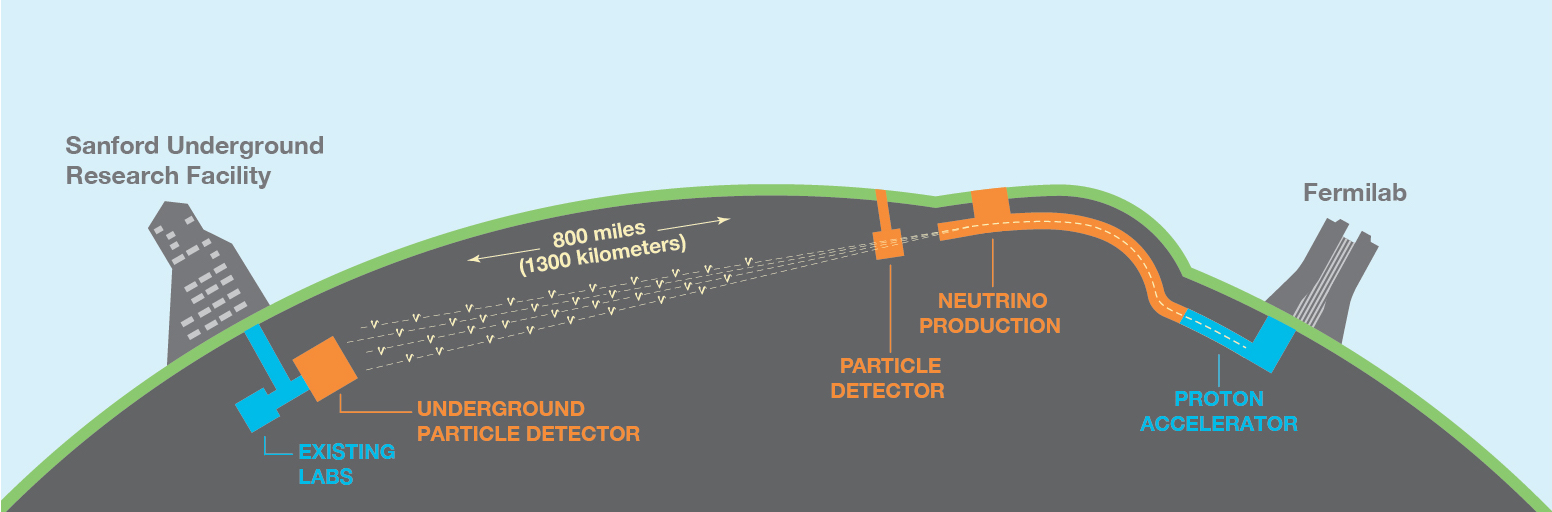
\includegraphics[width=120mm]{figures/dune.png}
  \caption{Cartoon of the DUNE setup \cite{DUNE_2020}}
  \label{dune}
\end{figure}

The plan is to have 2 sets of detectors, one at Fermilab, (near detector(ND)) and the other at SURF (far detector (FD)).
% https://arxiv.org/abs/2002.02967
The design of the DUNE far detector, grounded in cutting-edge Liquid Argon Time Projection Chamber (LArTPC) technology, is set to revolutionize particle physics.
This detector will be housed in a colossal volume of 70 kilotons of liquid argon, buried 1.5 kilometers underground \cite{DUNE_LBNF}.
To maximize the efficiency of physics experiments, the design splits this volume into four LArTPC modules, each with a usable "fiducial volume" of 10 kilotons, avoiding interactions near the edges.
To accommodate these massive detectors, approximately 800,000 tons of rock will be excavated, creating vast underground caverns.

The near detector will be built on the Argon cube concept.
The ND will have a modular design combined with a novel pixellated charge readout.
Previously, large detectors struggled with high demands for drift potentials and argon purity, which often led to risks of electric breakdown and purity losses.
By breaking down a large detector into smaller, independent modules, these risks are significantly reduced.
This modularity allows for easier maintenance and more reliable operation \cite{Biron_2020}.

\begin{figure}[H]
  % https://www.lhep.unibe.ch/research/detector_development/argoncube/index_eng.html
  \centering
  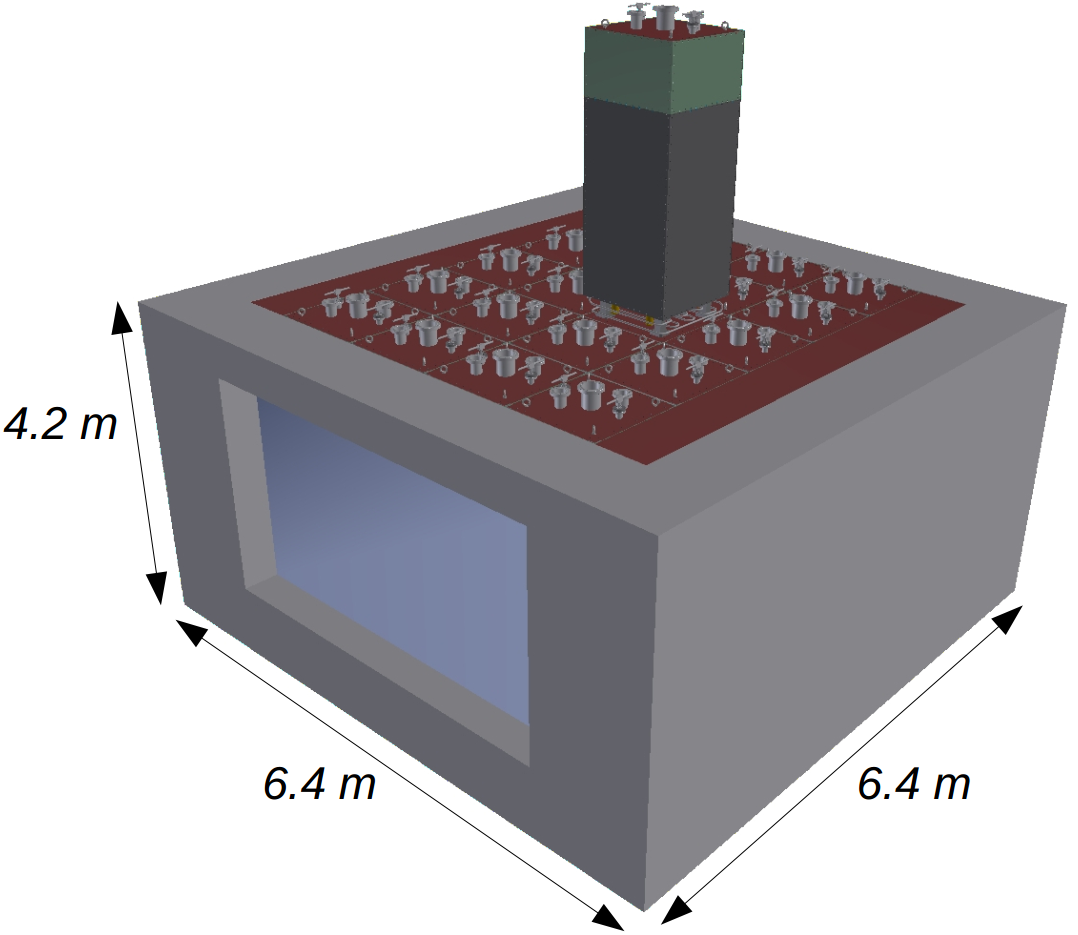
\includegraphics[width=80mm]{figures/nd.png}
  \caption{Design of the DUNE ND with $5 \times 7$ modules \cite{DUNE_2020a}}
  \label{nd}
\end{figure}

The fully pixelated charge readout adds another layer of sophistication, enabling precise event topology reconstruction.
This is important for handling high-multiplicity environments where pile-up could otherwise obscure important data.
Additionally, each module captures scintillation light to provide accurate timing information for neutrino events, further enhancing the detector's performance.

The real game-changer is the scalability of this design.
The modular approach means that the detector can be expanded to accommodate a very large active mass, opening up new possibilities for research and application.

\begin{figure}[H]
  % https://www.lhep.unibe.ch/research/detector_development/argoncube/index_eng.html
  \centering
  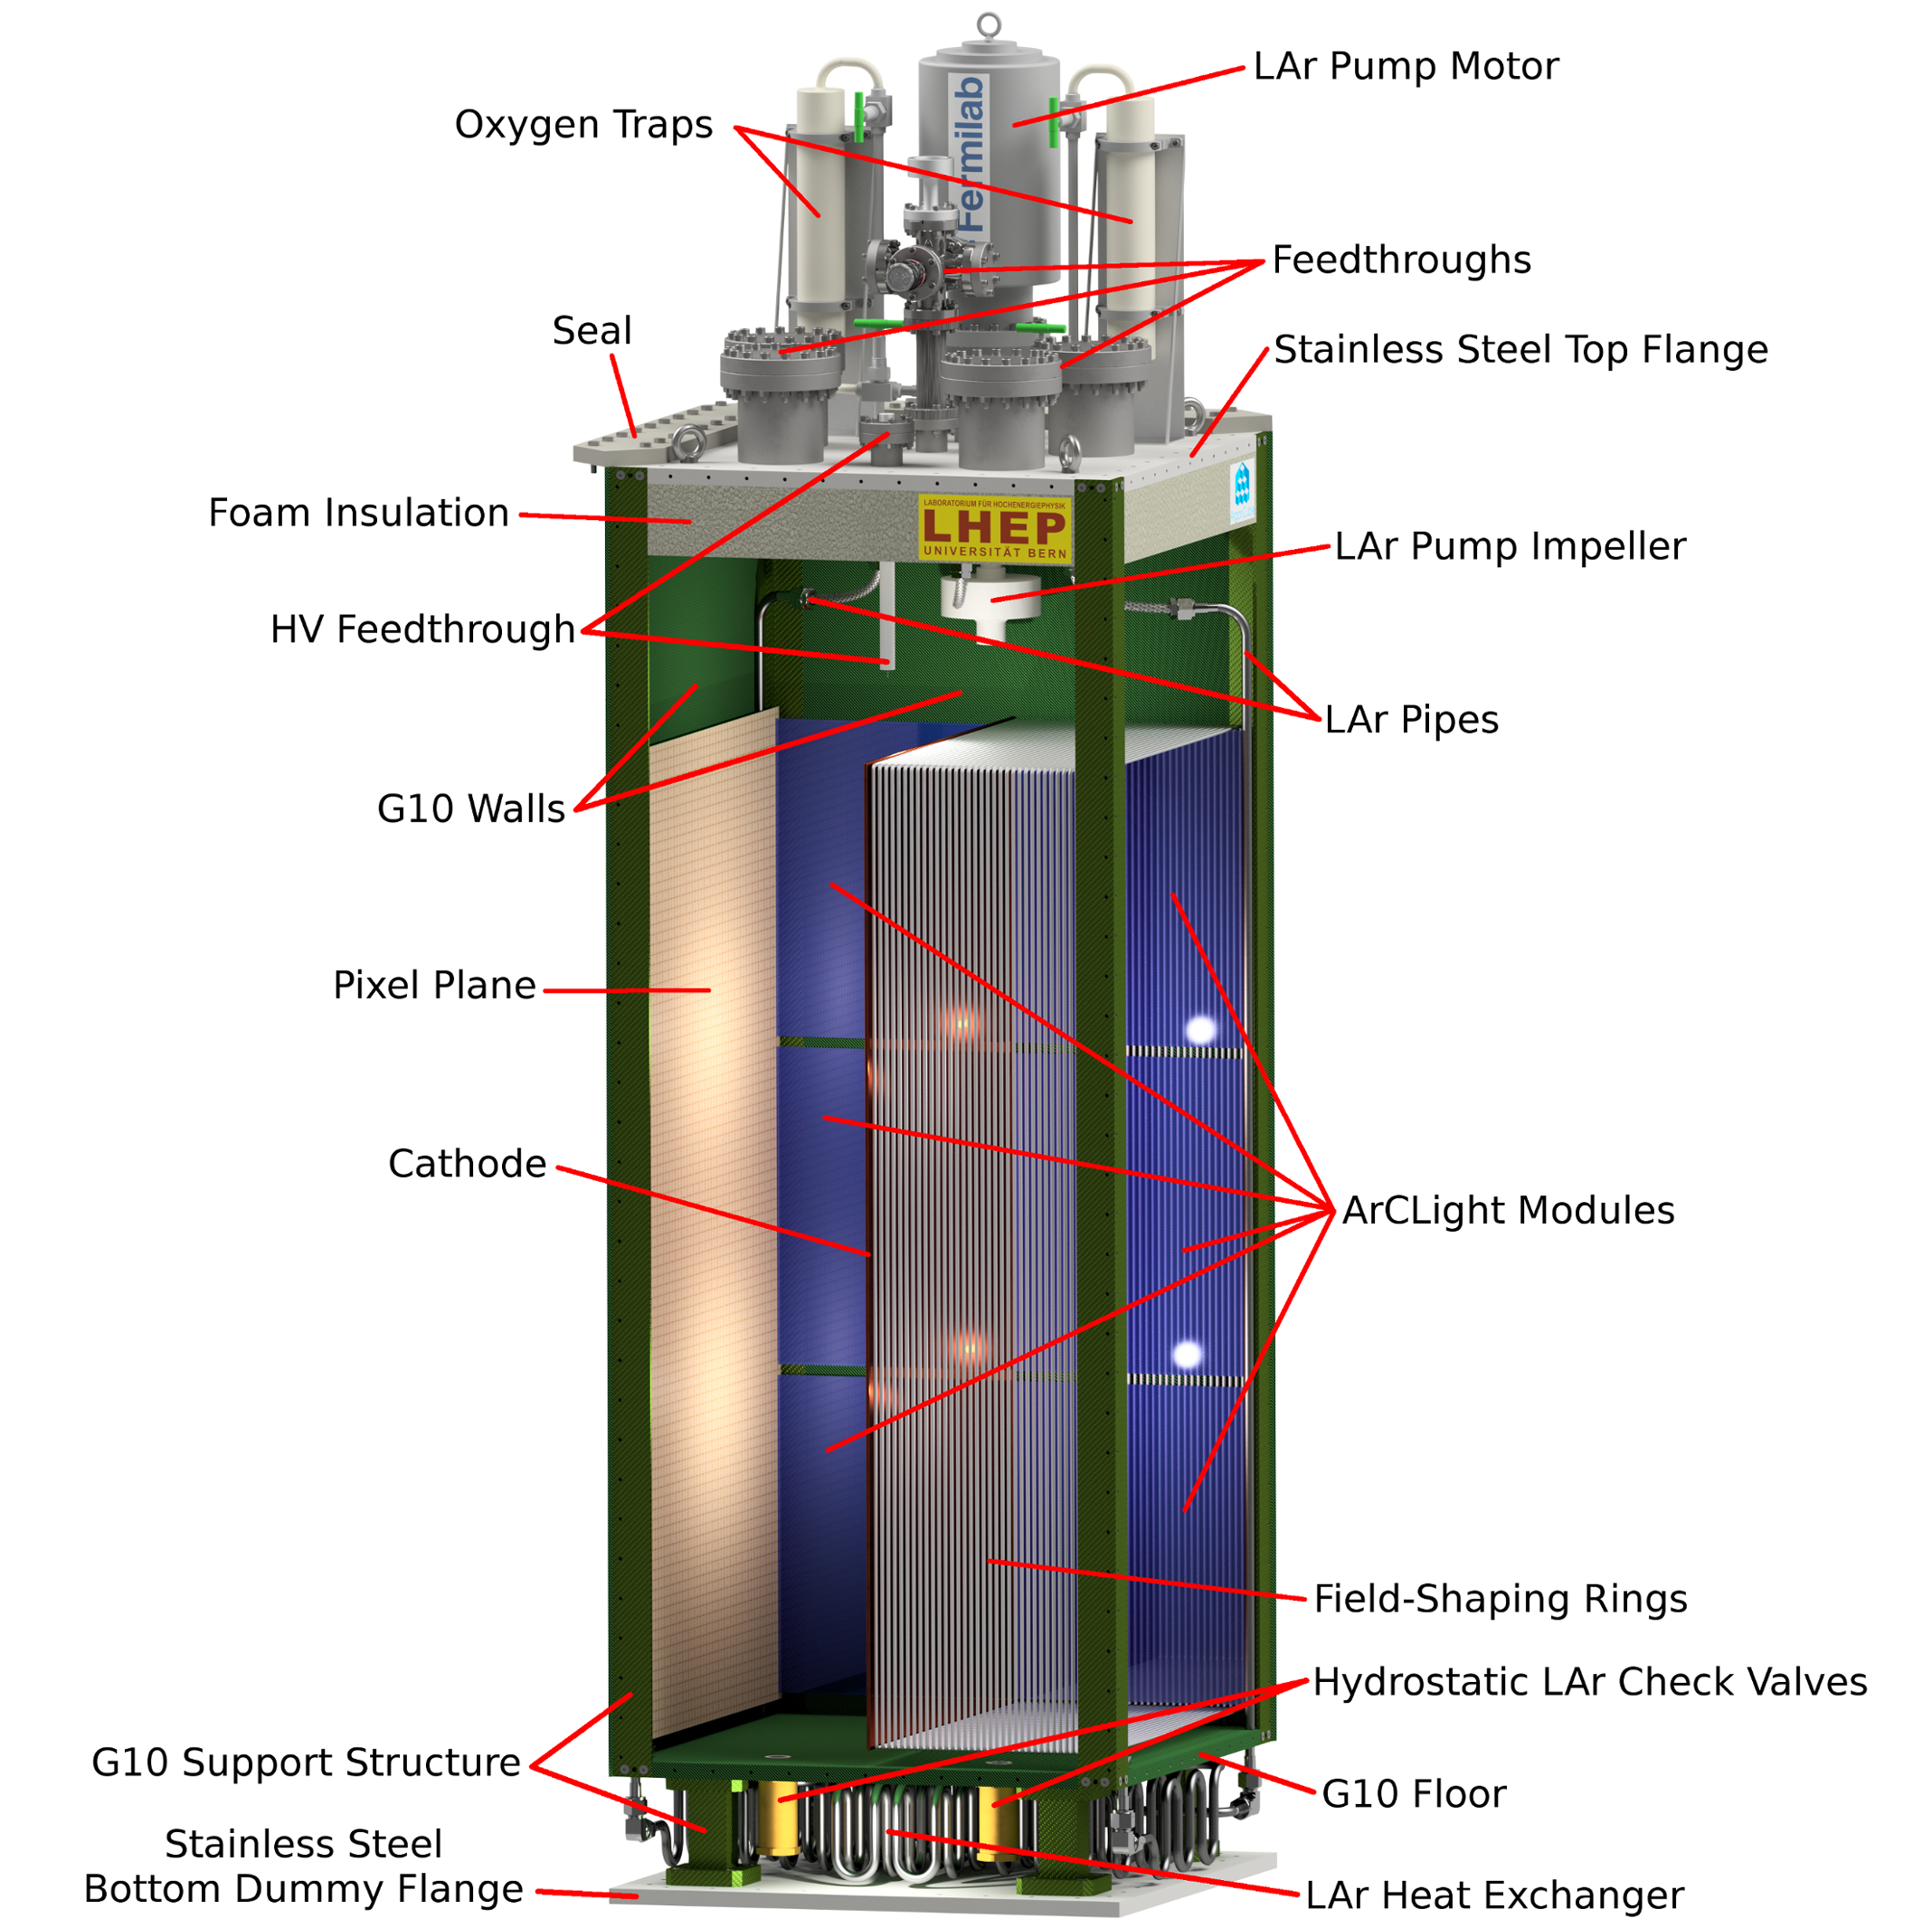
\includegraphics[width=80mm]{figures/ndModule.png}
  \caption{Cutaway image of a module\cite{DUNE_2020b}}
  \label{ndModule}
\end{figure}

Because of the novelty of the technology, a scaled down prototype  of the Argon cube detector called the $2 \times 2$ has been built.
Instead of having $5 \times7$ modules, it will have$2 \times 2$ modules.
Individual modules have already been built and tested before being put together to take data as part of a set.

\begin{figure}[H]
  % Original Image
  \centering
  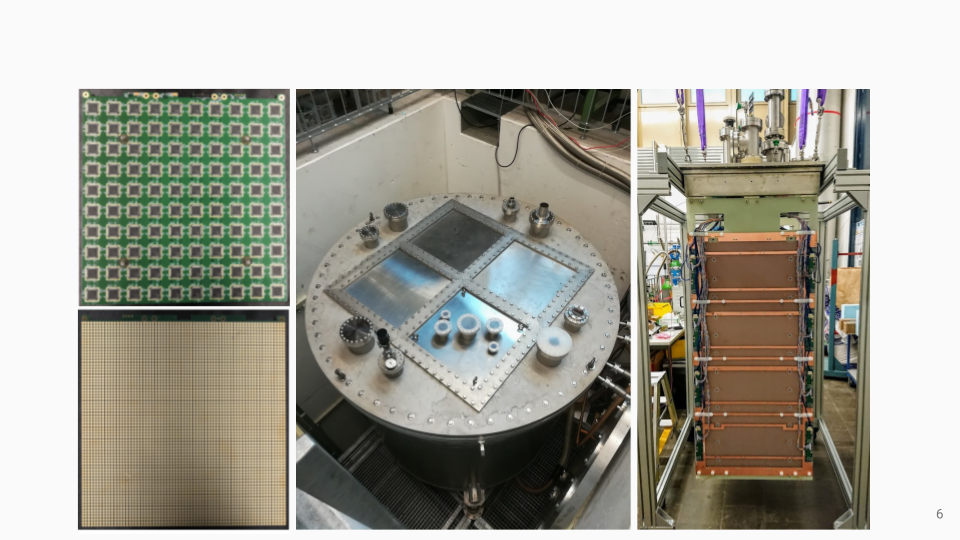
\includegraphics[width=120mm]{figures/ndPic.png}
  \caption{Pictures of the first module to be build (Module-0)}
  \label{ndPic}
\end{figure}

The scale of DUNE and its ambitious goals are reminiscent of the dramatic shifts in scientific paradigms brought about by the discovery of subatomic particles that challenged existing theories \cite{dune_tdr}.





